

\begin{example}\label{ex:PermuteScopeShallowFold}
The function
\begin{align*}
\ranked{\reduce k \Sigma\cdot \Gamma\to \reduce k (\Sigma\cdot \Gamma)}
\end{align*}
which puts shallow composition inside the scope of the fold is derivable. Indeed, it is the composition of the following functions:
\begin{align*}
\ranked{\reduce k \Sigma\cdot \Gamma\to \reduce k \Sigma\cdot \reduce k\Gamma^k\to \reduce k(\reduce k \Sigma\cdot \Gamma^k)\to \reduce k (\Sigma\cdot \Gamma)}
\end{align*} 
\end{example}

One annoying thing about the unfold function and the function that reduces the degree of the fold
\begin{align*}
\ranked{\tmonad \reduce k \Sigma \to \reduce k \tmonad \Sigma\cdot  \tmonad \reduce k \Sigma \qquad \reduce k\Sigma \to \reduce {k-l} {(\Sigma\cdot(0+1))}}
 \end{align*}
 is that they append a type after a $\cdot$. In our futur developments, we will need to derive functions of the form
 \begin{align*}
 \ranked{\Gamma\cdot\Delta\to \Gamma}
 \end{align*}
 to get rid of these appended types. Obviously, functions of this type are not derivable for any $\rGamma$ and $\rDelta$. We show in the following some situations where it becomes derivable.
 
 \begin{example}
 Suppose that $\rSigma$ is a ranked set containing a binary and a nullary element. We can derive a function
 \begin{align*}
\ranked{\tmonad\Sigma\cdot\Gamma\to \tmonad\Sigma}
 \end{align*}
 as the composition of the following functions:
 \begin{align*}
\ranked{\tmonad\Sigma\cdot\Gamma\to \tmonad\Sigma\cdot\bot\to\tmonad\Sigma\cdot\tmonad(0+2)\to \tmonad(\Sigma+0+2) \to \tmonad\Sigma} 
 \end{align*}

Suppose that $\rGamma, \rDelta$ are two types such that we can derive a function of type 
 \begin{align*}
 \ranked{\Gamma\cdot\Delta\to \Gamma}
 \end{align*}
Then we can also derive a function of type 
\begin{align*}
\ranked{\reduce k \Gamma\cdot\Delta\to \reduce k \Gamma}
\end{align*}
using the following derivation. 
\begin{align*}
\ranked{\reduce k \Gamma\cdot\Delta\xrightarrow{Ex.~\ref{ex:PermuteScopeShallowFold}} \reduce k (\Gamma\cdot\Delta) \to \reduce k \Gamma}
\end{align*}
Similarly, we can derive a function of type
\begin{align*}
\ranked{ \Gamma^k\cdot\Delta\to \Gamma^k}
\end{align*}
using the following derivation. 
\begin{align*}
\ranked{\Gamma^k\cdot\Delta\to (\Gamma\cdot\Delta)^k \to \Gamma^k}
\end{align*}
Using these functions, when we will want to reduce the degree of a fold of a type $\ranked{\tmonad\Sigma}$, $\ranked{(\tmonad\Sigma)^k}$, etc, we will use the following functions instead of the basic ones:
\begin{align*}
\ranked{\reduce l\tmonad \Sigma\to \reduce {l-m}(\tmonad \Sigma\cdot(0+1))\to \reduce {l-m}\tmonad \Sigma }\\
\ranked{\reduce l(\tmonad \Sigma)^k\to \reduce {l-m}((\tmonad \Sigma)^k\cdot(0+1))\to \reduce {l-m}(\tmonad \Sigma)^k }
\end{align*} 
\end{example}


\begin{example}[Partial shallow unfold]~\label{ex:PartialShallowUnfold}
We need a "partial shallow unfold"
\begin{align*}
\ranked{\reduce k \Sigma\cdot (1+\Gamma^k)\to \reduce k (\Sigma\cdot(1+\Gamma))}
\end{align*}
\begin{center}
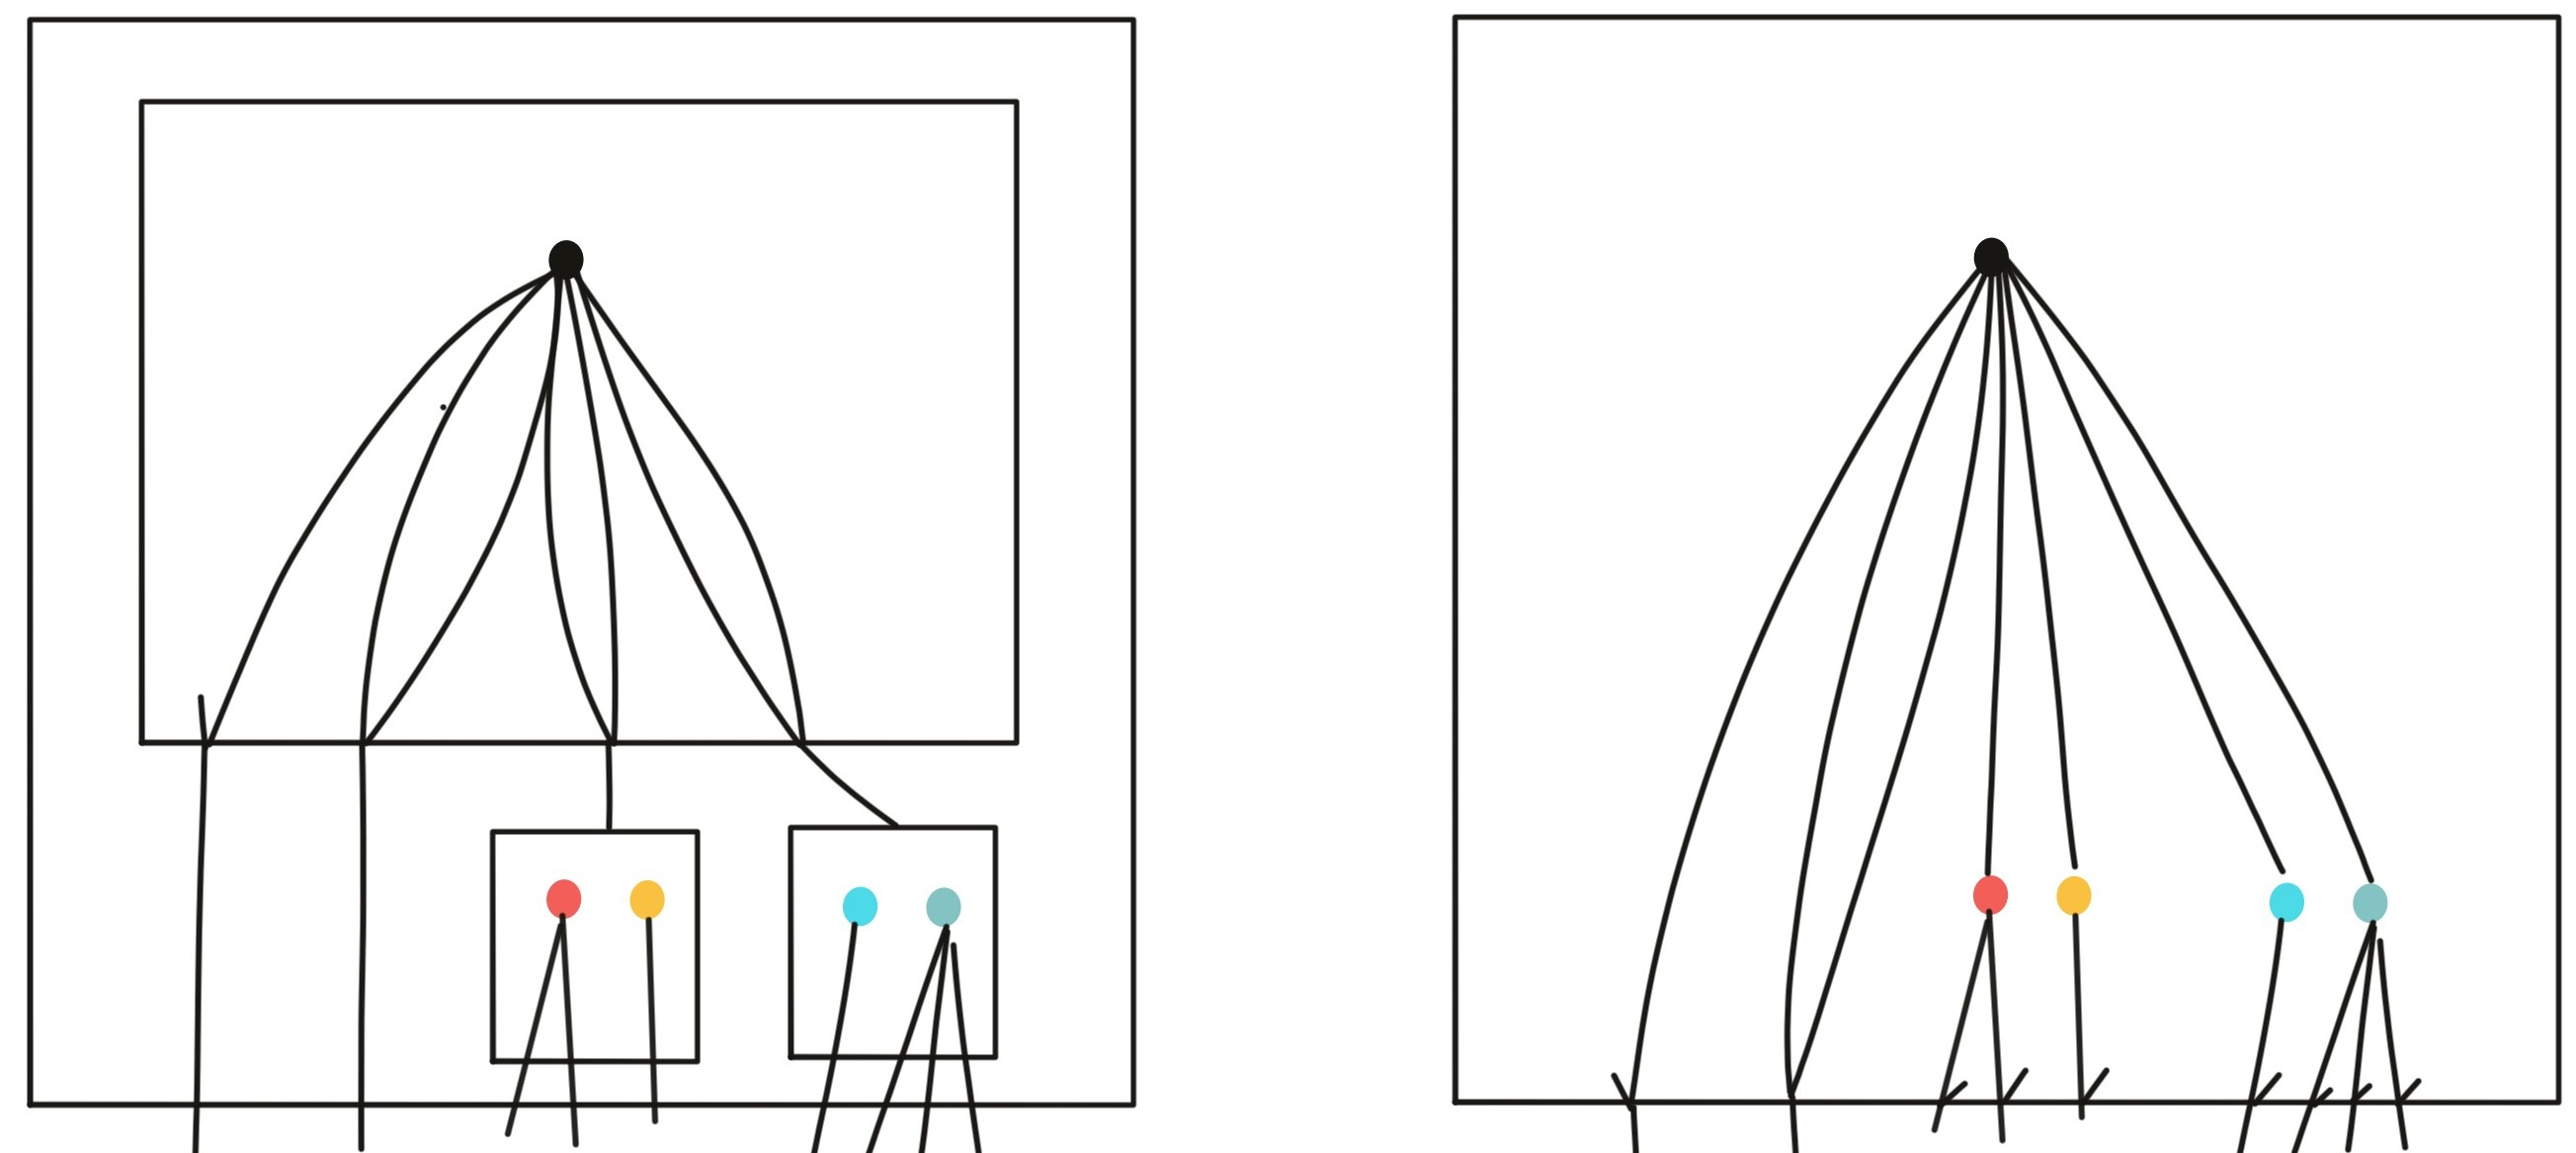
\includegraphics[scale=.09]{MyPicPartialShallowUnfold.jpg}
\end{center}
This function can be derived as follows. First we lift the functions
\begin{align*}
\ranked{1\to \reduce k 1^k}\qquad \text{ and } \qquad\ranked{\Gamma^k\to \reduce k\Gamma^k}
\end{align*}
obtaining the function
\begin{align*}
\ranked{\reduce k \Sigma\cdot (1+\Gamma^k)\to \reduce k \Sigma\cdot (\reduce k 1^k+\reduce k\Gamma^k) }
\end{align*}
We compose the result with the following  (series of) injections
\begin{align*}
\ranked{\reduce k \Sigma\cdot (\reduce k 1^k+\reduce k\Gamma^k)\to \reduce k \Sigma\cdot \reduce k (1+\Gamma)^k}
\end{align*}
Finally we permute the fold with the shallow product, then we apply the shallow unfold to obtain the result.
\end{example}

In order to prove lemma~\ref{lem:homo-twist}, we need to show that a very particular form of unfolding, which we call \emph{the unfolding of external twists}, is derivable. This function, which is of type 
\begin{align*}
\ranked{\tmonad \mati k \Sigma \to \reduce k \tmonad \mati k \Sigma}
\end{align*}
"untwists" the external twists  as illustrated by the following figure where the external twists have been colored in red. 
\begin{center}
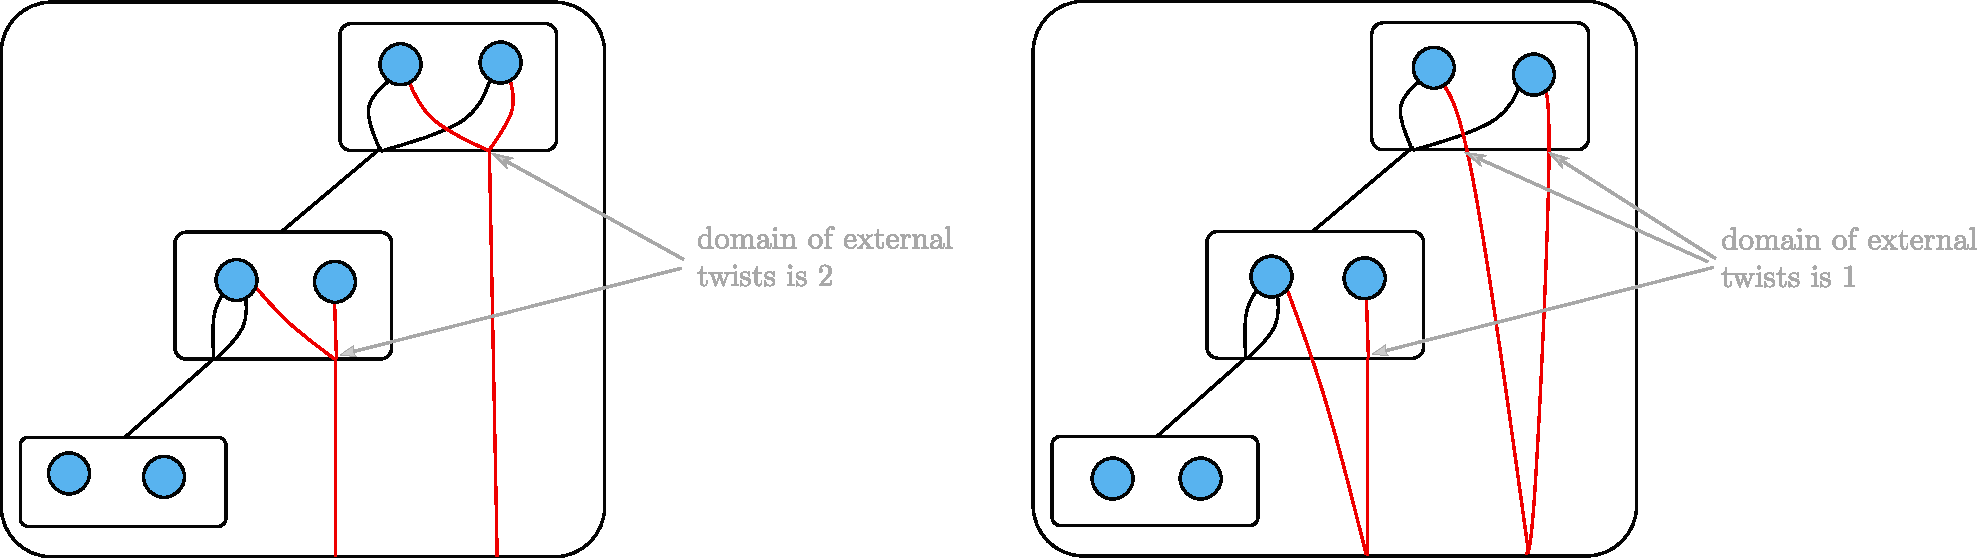
\includegraphics[scale=.4]{external-unfold.pdf}
\end{center}
The main feature of this function, which will be very useful later, is that the external twists of the output term have $1$ as domain.  


\begin{lemma}\label{lem:unfold-external-twist} If $u$ is an element of $\ranked{\reduce k \Sigma}$, let us denote by $\overline{u}$ the term of $\ranked{\Sigma}$ underlying it. There is a derivable function
\begin{align*}
\ranked{f:\tmonad \mati k \Sigma \to \reduce k \tmonad \mati k \Sigma}
\end{align*}
satisfying the following conditions:
\begin{itemize}
\item It preserves the unfolding. 
\item It preserves $\alpha$-homogeneity. That is, if $t\in\ranked{\tmonad\mati k \rSigma}$ is $\alpha$-homogeneous, so is $\overline{\ranked{f}(t)}$.
\item  For every term $t\in \ranked{\tmonad\mati k \rSigma}$, the domain of the external twists of $\overline{\ranked{f}(t)}$ is 1.
\end{itemize}
We call $\ranked{f}$ an external unfold function.
\end{lemma}
\begin{proof}
Let us derive a function $\ranked{f}$ satisfying the conditions of the lemma. We start by lifting to terms the following basic function 
$
\ranked{\mati k \Sigma  \to \mati k \Sigma \cdot1}
$.
After embedding the shallow terms into terms and performing a flattening, we get a term in $\ranked{\tmonad(\mati k\Sigma+1)}$. After that, we apply the function
\begin{align*}
\ranked{\tmonad(\mati k \Sigma+1)\to \tmonad(\mati k\Sigma+1+1)}
\end{align*}
which sends every node labeled by $1$ to the first copy if it is directly connected to the output, and to the second copy if not. This function is derivable as it can be implemented by an FO rational function. %We illustrate this by the following figure where the red nodes denote the first copy of $1$ and the blue nodes denote the second one
%\begin{center}
%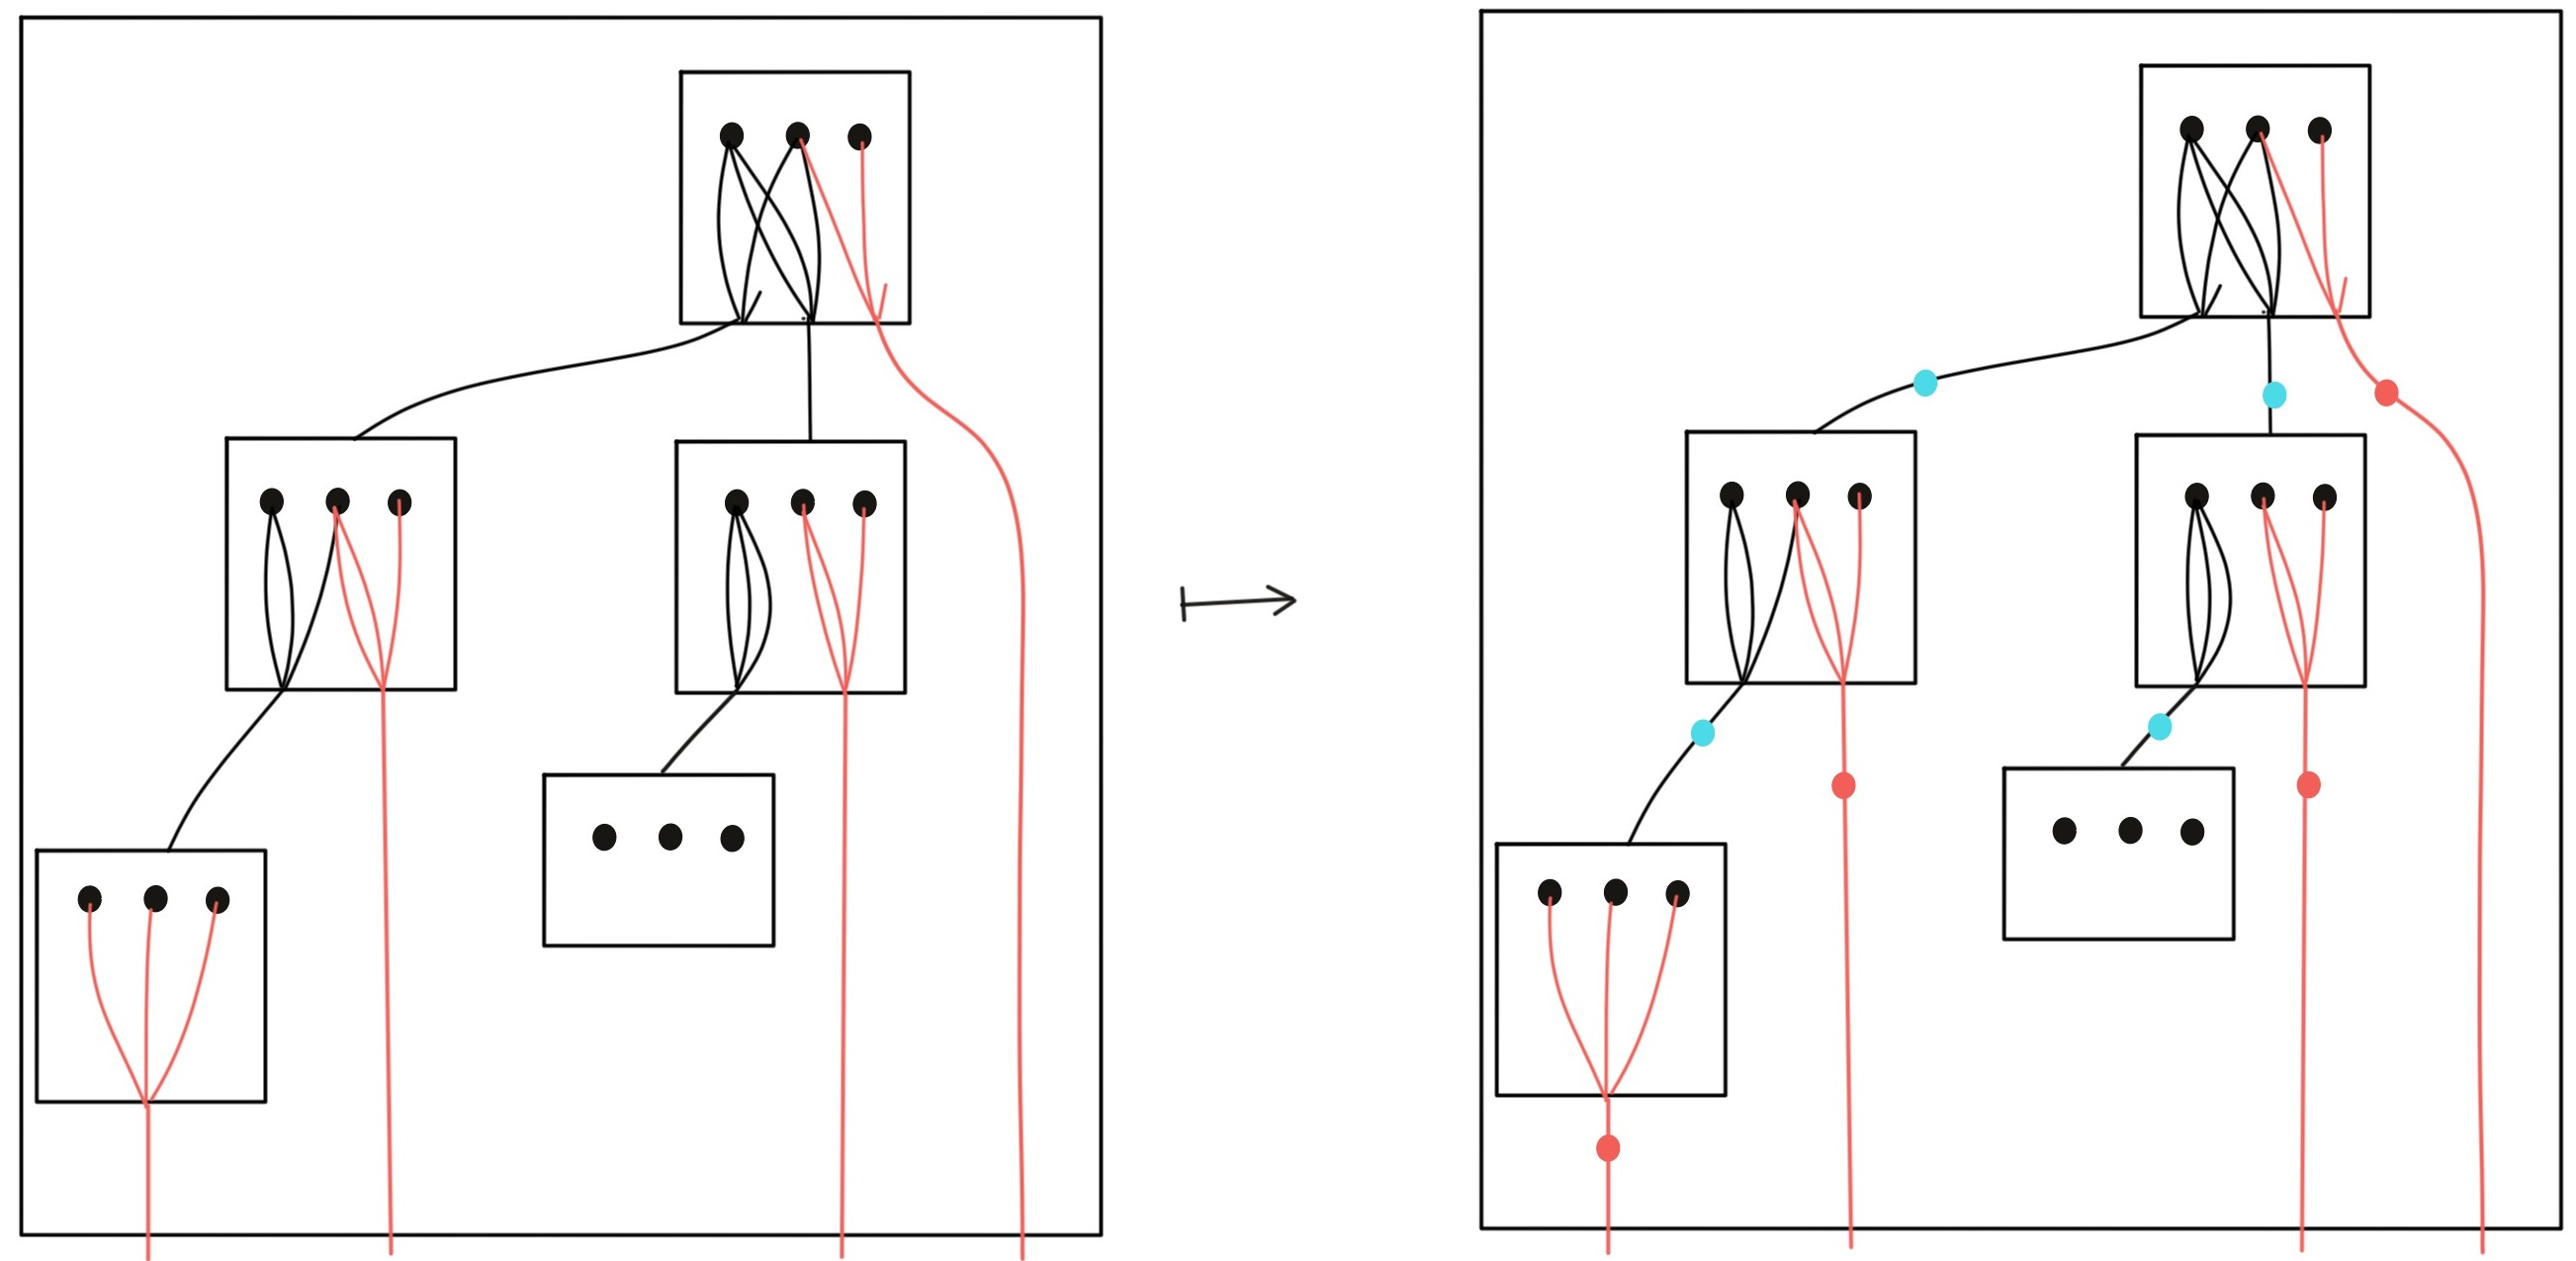
\includegraphics[scale=.1]{MyPicLabel1.jpg}
%\end{center}  
After that, we factorize the obtained term in such a way that each factor contains exactly a node $\ranked{\mati k \Sigma}$ with its children of type $\ranked{1+1}$. Such factorisation is of type
\begin{align*}
\ranked{\tmonad(\mati k \Sigma+1+1)\to \tmonad(\tmonad(\mati k \Sigma+1+1))}
\end{align*} 
and can be easily implemented using an fo rational function. The formed factors are of the form $\ranked{\mati k\Sigma\cdot(1+1)}$. We want to reflect that on the type, so that we can apply the basic functions of shallow terms. For that, we decompose $\ranked{\tmonad(\mati k \Sigma+1+1)}$ into $\ranked{\mati k \Sigma\cdot(1+1)+\bot}$ using the decomposition  function and the function 
that sends every type to $\ranked{\bot}$ to collect the ``garbage'' types.
Our term is now of type $\ranked{\tmonad(\mati k \Sigma\cdot(1+1)+\bot)}$. We apply the raising error function to get a term in $\ranked{\tmonad(\mati k \Sigma\cdot(1+1))+\bot}$.
Now, we lift the basic function
\begin{align*}
\ranked{\mati k \Sigma\cdot(1+1)\to \reduce k(\mati k \Sigma\cdot(1+1))}
\end{align*}
obtaining the following term of type $\ranked{\tmonad(\reduce k(\mati k \Sigma\cdot(1+1))+\bot)}$
\begin{center}
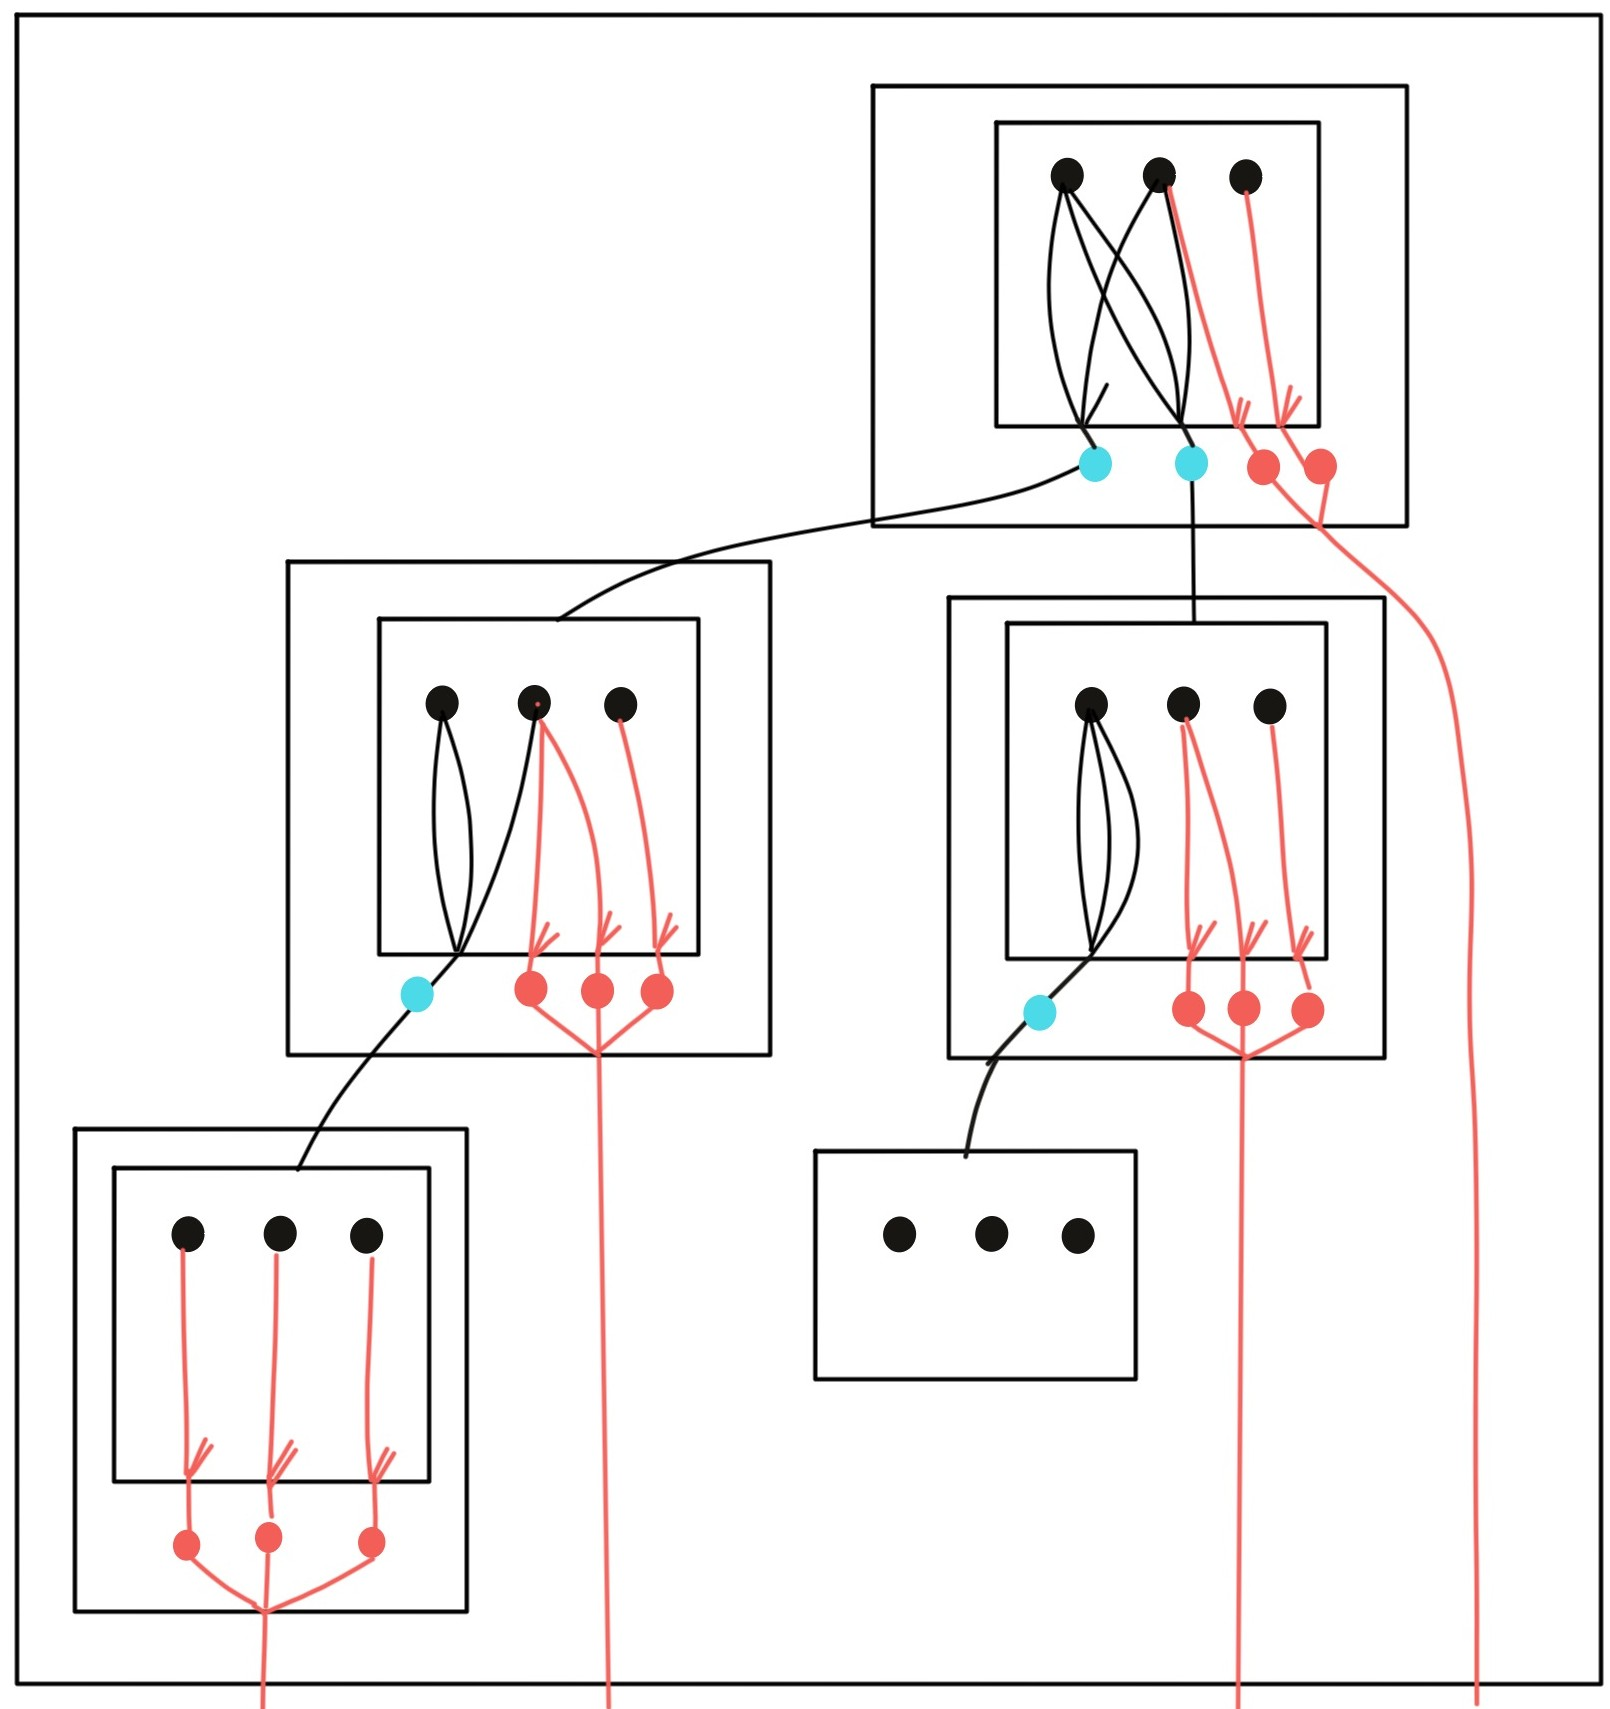
\includegraphics[scale=.1]{MyPic26.jpg}
\end{center}  
When we lift the functions $\ranked{1+1\to 1}$ and $\ranked{\mati k \Sigma\cdot 1\to \mati k \Sigma}$, we get a term in $\ranked{\tmonad(\reduce k \mati k \Sigma+\bot)}$ to which we apply the raise error function, followed by an unfolding, then by the function of Example~\ref{ex:ReduceDegreeRecoverType} which gets rid of the type after the $\cdot$.
\begin{align*}
\ranked{\tmonad(\reduce k \mati k \Sigma+\bot)\to \tmonad\reduce k \mati k \Sigma+\bot\to (\reduce k \tmonad\mati k \Sigma)\cdot\tmonad\reduce k \mati k \Sigma +\bot\to \reduce k \tmonad\mati k \Sigma+\bot }
\end{align*}
To obtain the desired type  we embed $\ranked{\bot}$ into $\ranked{\reduce k \tmonad\mati k \Sigma}$ using the fact that $\rSigma$ contains a nullary and a binary element. 

It is not difficult to see that the obtained function satisfies the conditions of the lemma.
\end{proof}